Here we have shown the result of our analysis, both intra procedural 
and loop sensitive, on some example codes. The goal of these preliminary 
experiments is to illustrate the accuracy of our method in the detection of 
dependences and to extract parallelism from heap intensive sequential codes. 
Codes, which only traverse the data structure and do not update or modify it, 
are main candidates for this analysis. Note that, statements of each code 
operating on heap are normalized and annotated with corresponding directives in the first step. 
For the reason of simplicity, we do not show them. The code from Figure~\ref{fig:treeadd} 
\begin{figure}%[t]
  \begin{center}
    \scalebox{.85}{\begin{tabular}{ c c }
      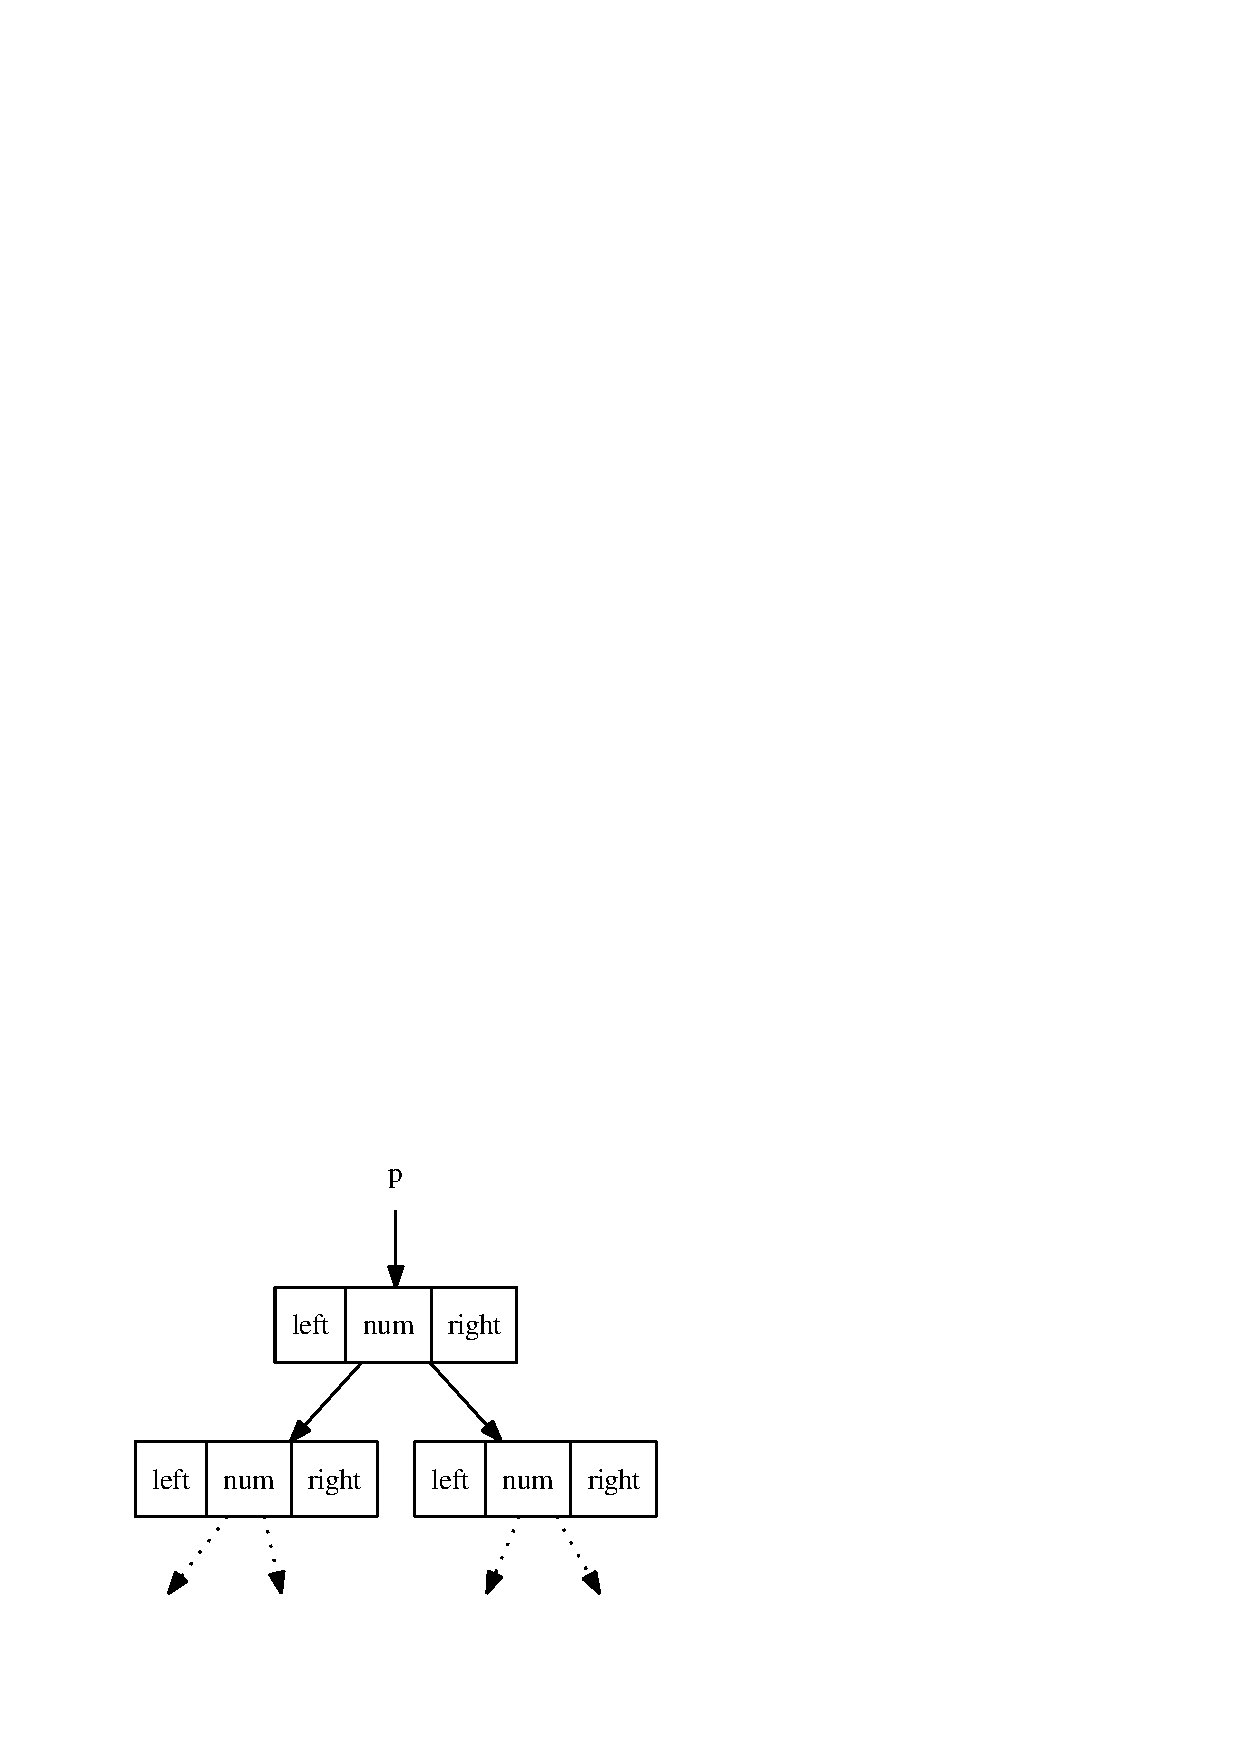
\includegraphics[scale=0.6]{grph_tree} %\cline{1-1}
      &
      {\tt
\begin{program}{0}
%  \FL\ \ldots
  \UNL{0} void treeAdd(tree t) \{
  \UNL{1}  if(t == NULL)
  \UNL{2} return;
  \NL{1}     tl = t$\rightarrow$left;
  \NL{1}     treeAdd(tl);
  \NL{1}     tr = t$\rightarrow$right;
  \NL{1}     treeAddd(tr);
  \UNL{1}	t\rtarrow{num} = tl\rtarrow{num} + tr\rtarrow{num};
  \UNL{0} \}
\end{program}
} \\
%      \includegraphics[scale=0.6]{grph_RD_WR} & \\
 %     (a) & (b) \\
  %    (a) Nodes read and written by code & 
  %    (b) Code fragment traversing the data structure. \\
    \end{tabular}}
  \end{center}
%  \hrule
  \caption{\label{fig:treeadd} Code fragment for \ttf{treeAdd} on tree data structure.}
%\hrule
\end{figure}
has taken to demonstrate the way our dependence analysis works for recursive function calls. 
As our  
%
%\begin{wrapfigure}{r}{0.5\textwidth}
%\begin{center}
%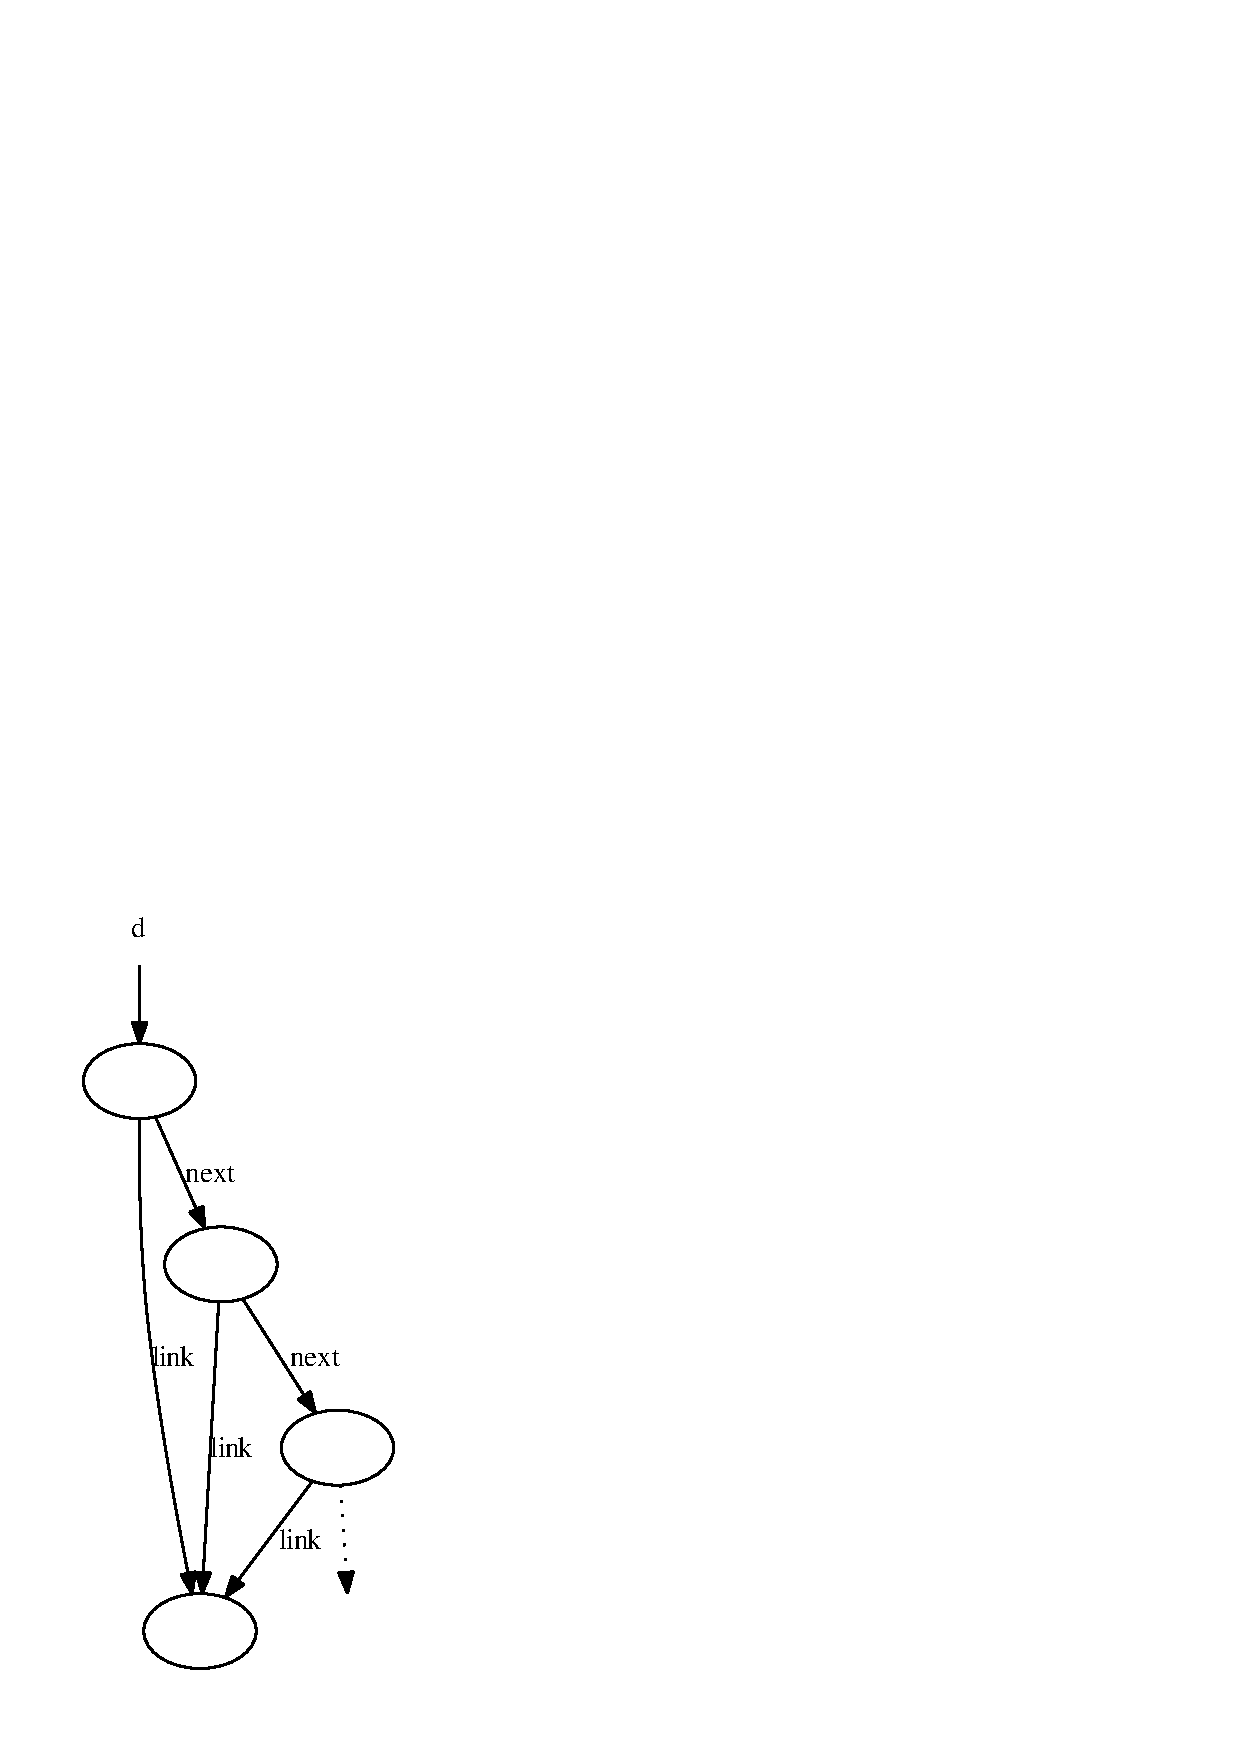
\includegraphics[width=0.26\textwidth]{grph_DAG}
%\end{center}
%\caption{A gull}
%\end{wrapfigure}
%
\begin{figure}%[t]
  \begin{center}
    \scalebox{.85}{\begin{tabular}{ c c c }
%      \includegraphics[scale=0.6]{grph_ex1} %\cline{1-1}
		{\tt
\begin{program}{10}
  \FL\ \ldots
  \UNL{0} p = d;
  \UNL{0} \WHILE (p\rtarrow{next} != NULL) \{
  \NL{1}   temp = p\rtarrow{num};
  \NL{1}   q = p\rtarrow{next};
  \NL{1}   q\rtarrow{num} = temp;
  \NL{1}     p = q\rtarrow{next};
  \UNL{0} \}
  \UNL{0} \ldots
\end{program}
} 
      &
      {\tt
\begin{program}{20}
  \FL\ \ldots
  \UNL{0} p = d;
  \UNL{0} \WHILE (p\rtarrow{next} != NULL) \{
  \NL{1}   temp = p\rtarrow{num};
  \NL{1}   q = p\rtarrow{link};
  \NL{1}   q\rtarrow{num} = temp;
  \NL{1}     p = p\rtarrow{next};
  \UNL{0} \}
  \UNL{0} \ldots
\end{program}
} \\
%      & {\tt
\begin{program}{20}
  \FL\ \ldots
  \UNL{0} p = d;
  \UNL{0} \WHILE (p\rtarrow{next} != NULL) \{
  \NL{1}   temp = p\rtarrow{num};
  \NL{1}   q = p\rtarrow{link};
  \NL{1}   q\rtarrow{num} = temp;
  \NL{1}     p = p\rtarrow{next};
  \UNL{0} \}
  \UNL{0} \ldots
\end{program}
} \\
    %  (a) & (b) \\
  %    (a) Nodes read and written by code & 
  %    (b) Code fragment traversing the data structure. \\
    \end{tabular}}
  \end{center}
%  \hrule
  \caption{\label{fig:motiv} Motivating example: (a)Nodes of data structure read(RD) and written(WR) by code, (b)Code fragment traversing the data structure. }
%\hrule
\end{figure}


In~\cite{Plevyak93analysisof} Plevyak et. al. present an analysis which depends on \emph{abstract storage graph} (ASG), an enhancement of Chase et. al.'s \emph{storage shape graph} (SSG)~\cite{Chase90}. Each node of SSG corrsponds to one or more nodes of runtime memory structure and the edges correspond to references. SSG algorithm is based on the heap reference counts, and cannot precisely handle singly linked list if muted and multiply linked structures. On the other hand, ASG models multiply-linked infinite structures and can efficiently handle structural modification of singly linked list. 




shape analysis::::::

\bb{Such informations are extensively used to 
detect memory leaks, for efficient garbage collection, parallelization etc. }

\bb{whose basic block is node consisting of one or more fields. Each field 
is designated as a scalar field or pointer field. A pointer field contains 
either value \emph{null} or pointer to a node of the same type. Unlike 
the scalar variable where the lvalue can be accessed directly, lvalue 
of a heap node can be obtained by traversing over the structure recursively. 
The organisation of such structures can be identified by shape analysis. }
